\section{Implementation}

\subsection{About Ngene}
\emph{Ngene} is a flexible, generic, multipurpose genetic algorithm written in C++ with heavy emphasis on performance and flexibility. The engine is divided into logical modules that can be interchanged or extended upon in order to fit the intended goal and purpose.

\subsubsection{Modular Design}
The design is broken into the following modules:

\begin{itemize}
	\item (core) - The genetic algorithm itself
	\item Fitness - Assesses the fitness of a genotype
	\item Genotype - Produces the genotype and translates them to phenotype
	\item Mating - Crosses two genotypes
	\item Mutator - Mutates a genotype
	\item Selector - Selects a random genotype
\end{itemize}

Of these modules, only the core, or the genetic algorithm itself, is currently not interchangeable though this might be changed in the future. All modules are loaded into memory when the program is executed and kept there until termination. This modular design is essential when it comes to making the engine available for all purposes. For example, while the \emph{tournament} selection module is suitable for most of the experiements in this thesis, others may want to run a comparison test between many selection modules. This is easily done by simply specifying which module to use in a configuration file. There is no need to recompile a single line of code. This modular design also keeps the code cleaner and easier to maintain.

\subsubsection{Boost C++ Libraries}
\emph{Boost}\footnote{\url{http://www.boost.org/}} is a collection of libraries that is meant to complement the C++ Standard Library. Ngene makes use of this collection in order to solve problems others already have. This not only saves time and effort, it also guarantees that a certain piece of code works as it should.

\paragraph{\textbf{Boost.Any}}\cite{henney2001}
A problem with writing a generic genetic algorithm in a strongly typed programming language as C++, is that different studies require different data types to be passed around the system. A simple program that sorts numbers, for instance, needs to pass around an array with integers while another one may require the use of a class or custom datatype. In a higher level language such as Python, a container is already available that can store any type of data:

\begin{verbatim}
>>> foo = 1 + 2
>>> print foo
3
>>> foo = "awesome"
>>> print foo
awesome
>>> _
\end{verbatim}

Such a container is unfortunately not readily available in C++ and must be implemented in order for the modular design to work. Fortunately, this has already been done and is freely available as part of \emph{Boost}. \emph{Boost.Any} is a container not very different from the one found in Python and only requires a type-casting before the data can be handled as normal.

\paragraph{\textbf{Boost Random Number Library}}\cite{maurer2000}
Another problem with genetic algorithms and development in general is implementing a good pseudo-random number generator. This is pretty much required to achieve good results. Ngene uses the implementation of \emph{Mersenne twister} pseudo-random number generator found in the Boost libraries.

\subsubsection{Brief System Overview}
\begin{figure}[ht]
	\centering
	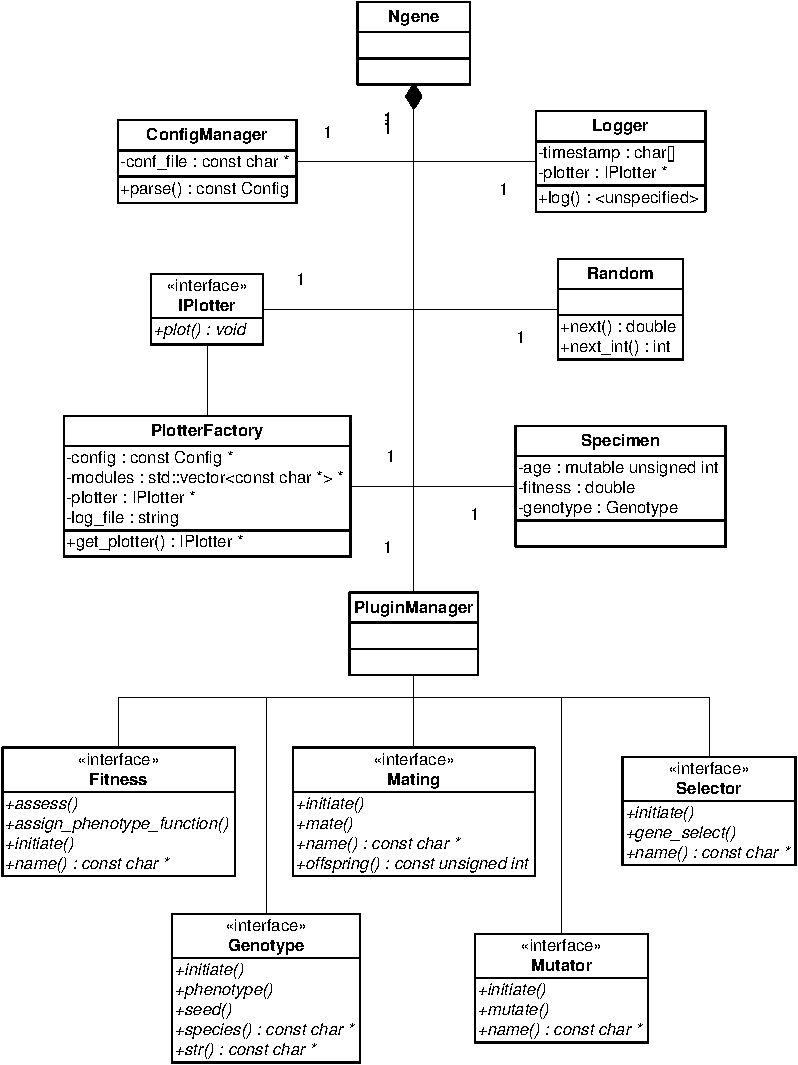
\includegraphics[scale=0.9]{diagram_ngene}
	\caption{Overview of Ngene}
	\label{fig:diagram_ngene}
\end{figure}

Figure~\ref{fig:diagram_ngene} shows a brief overview of how Ngene is put together.

When the program starts up, Ngene will start parsing a configuration file. It finds this file either via the path passed as parameter on execution, or it will simply start looking for the default one. The module responsible for this, \texttt{ConfigManager}, will create a structure storing the configuration and pass it to \texttt{PluginManager}.

\texttt{PluginManager} handles all loading and unloading of modules specified in a configuration file. If all modules load successfully, it also acts as an interface through which the core communicates with the modules. In future versions, there may be a possibility to swap modules, for instance, half way through an evolution. \texttt{PluginManager} will automatically unload modules and release all resources when it is destroyed on program exit.

Ngene talks with its modules via pre-defined interfaces as can be seen directly under \texttt{PluginManager} in figure~\ref{fig:diagram_ngene}. All methods in these modules must be implemented in order to be compatible with Ngene. A more detailed description of what these methods do and sample code can be found in the system documentation. Besides these restrictions, a user can extend the system in any way they see fit.

All logging of runs are done in \texttt{Logger}. On first call, it will make sure that the user has writing privileges and, on successive calls, plot a graph of the progression. When the program terminates, it will also create a file output of the best specimen. The format of this file is left to the author of the \texttt{Genotype} module. It could be anything from a simple text file to a proprietary format. At writing moment, \texttt{Plotter} only saves the graphs as SVG\footnote{Scalable Vector Graphics - \url{http://www.w3.org/Graphics/SVG/}} though other formats can be easily added.

The genetic algorithm starts by populating the adult population, a responsibility of the \texttt{Genotype} module. The randomly generated genotypes are stored in \texttt{Specimen}s in an array, or vector, that will make up the adult population. When this vector is full (a configurable value), the genetic algorithm will run for a given number of generations (also configurable) or until a perfect \texttt{Specimen} is found, e.g. \texttt{fitness = 1.0}.


\subsection{Ngene Development Framework}
\begin{figure}[ht]
	\centering
	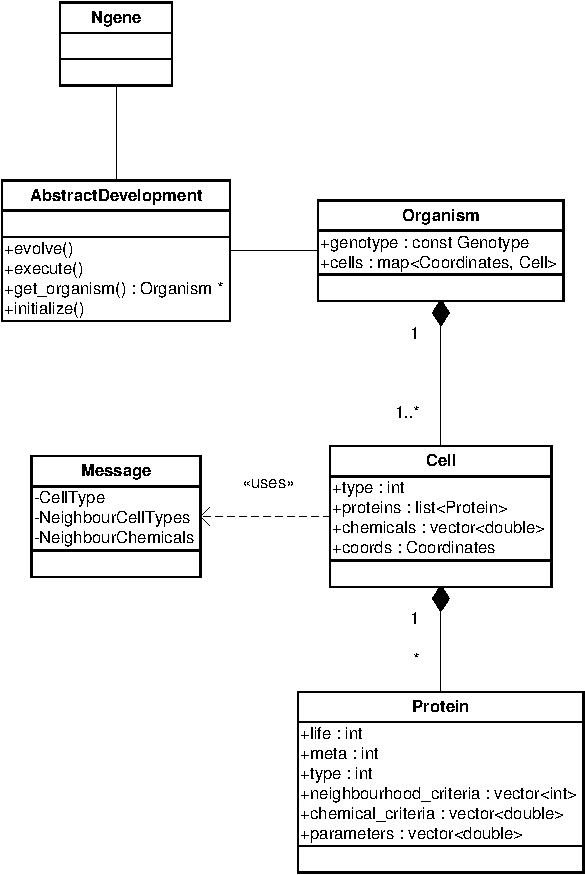
\includegraphics[scale=0.9]{diagram_ndevframe}
	\caption{Overview of Ngene Development Framework}
	\label{fig:diagram_ndevframe}
\end{figure}

To further extend the genetic algorithm already implemented in Ngene, a generic development framework has also been put into place. This framework consists of an abstract class that must be implemented and a few pre-defined classes that the user has to use (see fig.~\ref{fig:diagram_ndevframe}). This is to ensure that different development models will have a common ground on which it will be easier to compare one to another. The \texttt{Organism} and its ``components'', \texttt{Cell} and \texttt{Protein}, are meant to do exactly this. A common base code will eliminate factors that may influence a comparison. A \texttt{Message} class is also available for information exchange between all \texttt{Cell}s (see fig.~\ref{fig:diagram_ndevframe_msg}).

\begin{figure}[ht]
	\centering
	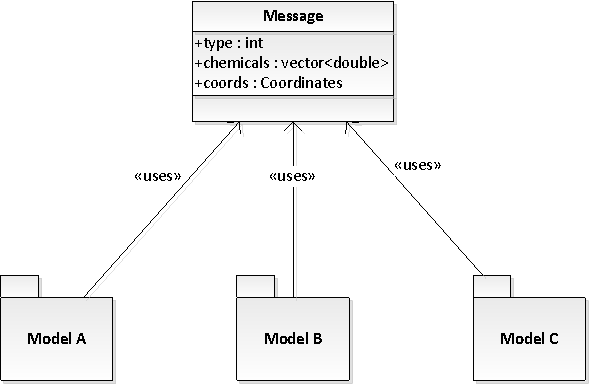
\includegraphics[scale=0.9]{diagram_ndevframe_msg}
	\caption{A common message implementation should eliminate factors involving what information is exchanged between the organism's cells.}
	\label{fig:diagram_ndevframe_msg}
\end{figure}

A module can be created by inheriting \texttt{AbstractDevelopment} and implementing the required methods, \texttt{execute()} and \texttt{initialize()}. The latter is executed everytime a new organism is to be developed and used to instantiate initial values for the organism like creating the zygote. \texttt{execute()} is called every tick and is used to exchange cell messages, update cells, and perform cell program. For an example, see figure~\ref{fig:diagram_ndevframe_ex}.

\begin{figure}[ht]
	\centering
	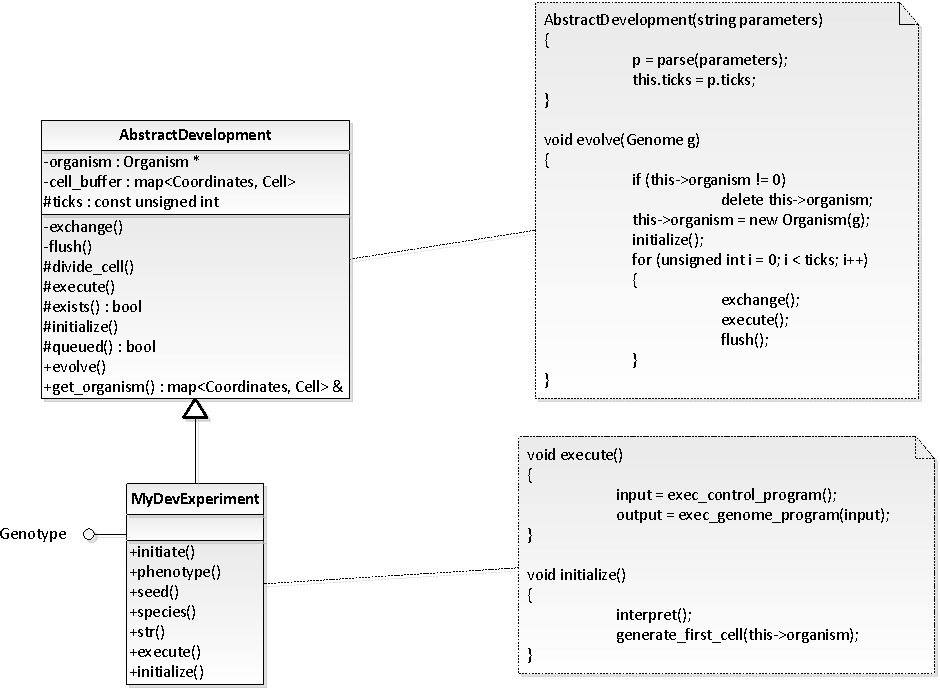
\includegraphics[scale=0.9]{diagram_ndevframe_ex}
	\caption{An example of how one can implement \texttt{MyDevExperiment}.}
	\label{fig:diagram_ndevframe_ex}
\end{figure}


\subsubsection{Johan H{\o}ye's Model}
A simpler (and hopefully faster) version of Johan H{\o}ye's master's thesis\cite{hoye2006} model was implemented with the help of the framework. Though simpler, all logical operations are still kept intact and was not altered in any way.

Due to lack of documentation, porting his code from Java to C++ has been a rather dirty job. Many biology concepts made their way into his code, making it very messy and difficult to read at times. There are classes for pretty much every concept such as \texttt{Cell}, \texttt{Protein} and even \texttt{Proteincollection} and \texttt{ChangeChemicalConcentrationInCellProtein}. Because of how the hierarchy is built up, functions may call other functions which again call different functions, and so on, to perform simple operations. These functions are often called many times in a single cell during a single tick, putting a strain on the call stack when there are a lot more cells in an organism, more ticks in a development process, and many organism in a population that are to evolve over generations. Parts of the effort in porting this model over to the new framework has been spent on flattening the structure a bit, hopefully making it simpler and easier to understand. In many cases, it was simply substituting a class, such as \texttt{Chemicalconcentrations}, with an STL container. After all, the golden rule of programming is to not write custom containers unless deemed absolutely necessary.

There are a couple of issues that Johan may have missed when he wrote his thesis. A lot of papers in this field agree to a certain degree that cells develop simultaneously, i.e. for all development that is based on neighbouring cells' states, an information exchange between all cells should occur first, and any other cellular operations last. However, in Johan's model, this is not implemented. The following snippets from his code should demonstrate this issue.

\begin{verbatimtab}
development/model/DevelopmentProsess.java:287-307:

/*
 * Performs a tick.
 * The development prosess steps one step forwards.
 */
private boolean doTick() {
	int cTime = getCurrentTick();
	int dTime = this.numberOfTicks;
	boolean success = false;

	if(cTime < dTime) {
		[...]
		this.currentOrganism.tickEvent(); //< Development occurs here
		this.currentTick++;
		success = true;
	} else {
		setActive(false);
	}
	return success;
}
\end{verbatimtab}

A tick signalises the organism to start doing something. Here, a tick event is triggered in an organism a certain amount of times.

\begin{verbatimtab}
development/model/framework/organism/Organism.java:90-101:

/**
 * Informs all cells in this organism of a tick event.
 * Each time this method is called, the development proceeds one step.
 * This method should be called each time a tick happens in
 * {@link DevelopmentProsess}
 */
public void tickEvent() {
	[...]
	// notify each cell of the tick
	for (Cell c : cells) {
		c.tickEvent();
	}
}
\end{verbatimtab}

The organism receives the event and then relays this tick event to all cells inside of it. This occurs in the order in which the cells were added to the array.

\begin{verbatimtab}
development/model/framework/cell/Cell.java:275-293:

/**
 * Handles the actions this cell must do each tick.
 * The order in which the different processes are carried out may have a great
 * effect on the behaviour of the cell. Great care must be taken if changing
 * this method!
 *
 */
public final void tickEvent() {
	[...]

	// Clears all requested actions
	resetRequestedActions();

	// This cells protein collection is doing their action
	pc.tickEvent();

	// This cell is doing its action
	doAction();
}
\end{verbatimtab}

Here we see that all requested actions by this cell's proteins are deleted before new actions can be requested. This happens in \texttt{pc.tickEvent()}: First, all dead proteins are removed from the collection and the remaining are aged. Finally, these proteins can request an action upon the cell based on chemical levels in the cell, as well as criteria based on neighbouring cells' types. These queued actions are accumulated and realised in \texttt{doAction()}.

We see that \texttt{Cell.tickEvent()} performs both the information gathering and all the actions as a single function while they should've been split up and run in two different loops. The problem here is that a single cell may get ``newer'' information from a neighbouring cell that already has been processed mixed up with ``older'' information from unprocessed cells, what it should've based its actions on.

For the purpose of my thesis, \texttt{doAction()} has been extracted out of \texttt{Cell.tickEvent()} and is called separately in another loop. This may or may not have a consequence in the outcome of the runs. The experiments conducted will show whether or not this is the case.


\subsubsection{Julian F. Miller's Model}
This model is based a number of works such as \cite{mteurogp2000} and \cite{ecal2003}. There are no official documentation or source code of it, so all work is based solely on descriptions of how it works.
